The fog grows thinner the further you climb. At the top of the ascent, you’re finally able to make sense of your surroundings--and the full extent of their destruction. The block's entire exterior wall has been torn away, along with much of its third floor and foundation. The mezzanine level ends in a sheer cut overlooking a fog-choked riverside.\\

Something stirs, drawing your attention to a nearby heap of rubble. The man-height semi-circle was not merely the chance product of a crumbling ceiling. Its construction looks to have been purposeful. Pacing around its opening, you discover two dozen or so burnt corpses piled within. So that's where the block's prisoners ended up--as a macabre sort of nesting material.\\

%%%

Circling within full view of the nest's entrance, it becomes obvious what’s making its home there: something of a cross between a man and a dead tree. It is rooted in the midst of the dead, its pale, fleshy branches quivering slightly. Its body pulses with a red glow, as if a hearth had been kindled in its belly. And when it lets out a scream, a jet of flame erupts from its jagged mouth.

\subsection*{Victory Condition}
Defeat the Thing From the Fog

\begin{tcolorbox}
\subsection*{Doom Events}
\begin{itemize}
\item \textbf{Every 3rd Round:} \emph{The Thing coughs and sputters, its body pulsing with a menacing glow.} For this Round, the \emph{Belch Fire} attack is replaced by \emph{Roaring Jet}.
\end{itemize}
\end{tcolorbox}

\subsection*{Encounter Table}
\begin{tcolorbox}
\textbf{Roll:} 2D6
\begin{center}
\begin{tabular}{ L | L | L }
\multicolumn{1}{c|}{\textbf{2}} & 
\multicolumn{1}{c|}{\textbf{3}} & 
\multicolumn{1}{c}{\textbf{4-5}} \\
\textbf{A:} \emph{Choke Slam}\newline \textbf{B:} \emph{Belch Fire} &
Move. \emph{Lunge} &
\textbf{A:} \emph{Belch Fire}\newline \textbf{B:} Move. Move \\
\hline
\multicolumn{1}{c|}{\textbf{6}} & 
\multicolumn{1}{c|}{\textbf{7}} & 
\multicolumn{1}{c}{\textbf{8}} \\
\textbf{A:} Move. \emph{Swipe}\newline \textbf{B:} \emph{Swipe. Lunge} &
\textbf{A:} \emph{Swipe. Lunge}\newline \textbf{B:} Move. \emph{Swipe} &
\textbf{A:} Move. \emph{Swipe}\newline \textbf{B:} \emph{Swipe. Lunge} \\
\hline
\multicolumn{1}{c|}{\textbf{9-10}} & 
\multicolumn{1}{c|}{\textbf{11}} & 
\multicolumn{1}{c}{\textbf{12}} \\
\textbf{A:} \emph{Belch Fire}\newline \textbf{B:} Move. Move &
Move. \emph{Lunge} &
\textbf{A:} \emph{Choke Slam}\newline \textbf{B:} \emph{Belch Fire}
\end{tabular}
\end{center}
\end{tcolorbox}

\subsection*{Enemy Sheet}
\hrule
\ \\
{\large \textbf{Thing From the Fog}}\\\\
\begin{tabular}{s s s}
\textbf{HP:} 16 & \textbf{Move:} 2\\
\textbf{P.DEF:} 1 & \textbf{F.DEF:} 2 \\
\end{tabular}\\

\emph{Hollow:} This entity ignores the Charmed, Maddened, and Fear conditions.\\

\emph{Sturdy:} This entity is immune to Knockback.\\

\emph{Bloodless:} This entity is immune to Bleeding and Bleed damage.\\

\textbf{Attacks:}
\begin{itemize}
\item \emph{Swipe} -  Deal 2 \emph{Unparryable} Slash damage to an adjacent entity.
\item \emph{Lunge} - Move 1. Deal 1 \emph{Unparryable} Crush damage and inflict Knockback 1 on an adjacent entity.
\item \emph{Choke Slam} - Deal 2 \emph{Unparryable} Crush damage and inflict Knockdown on an adjacent entity.
\item \emph{Belch Fire} - Deal 1 Burn damage to an entity that is within 3 tiles.
\item \emph{Roaring Jet} - Deal 1 \emph{Undodgeable} Burn damage and inflict Blazing in a 3-hex cone.
\end{itemize}
\hrule
\ \\

\pagebreak

\subsection*{Encounter Map}
\begin{center}
\framebox{
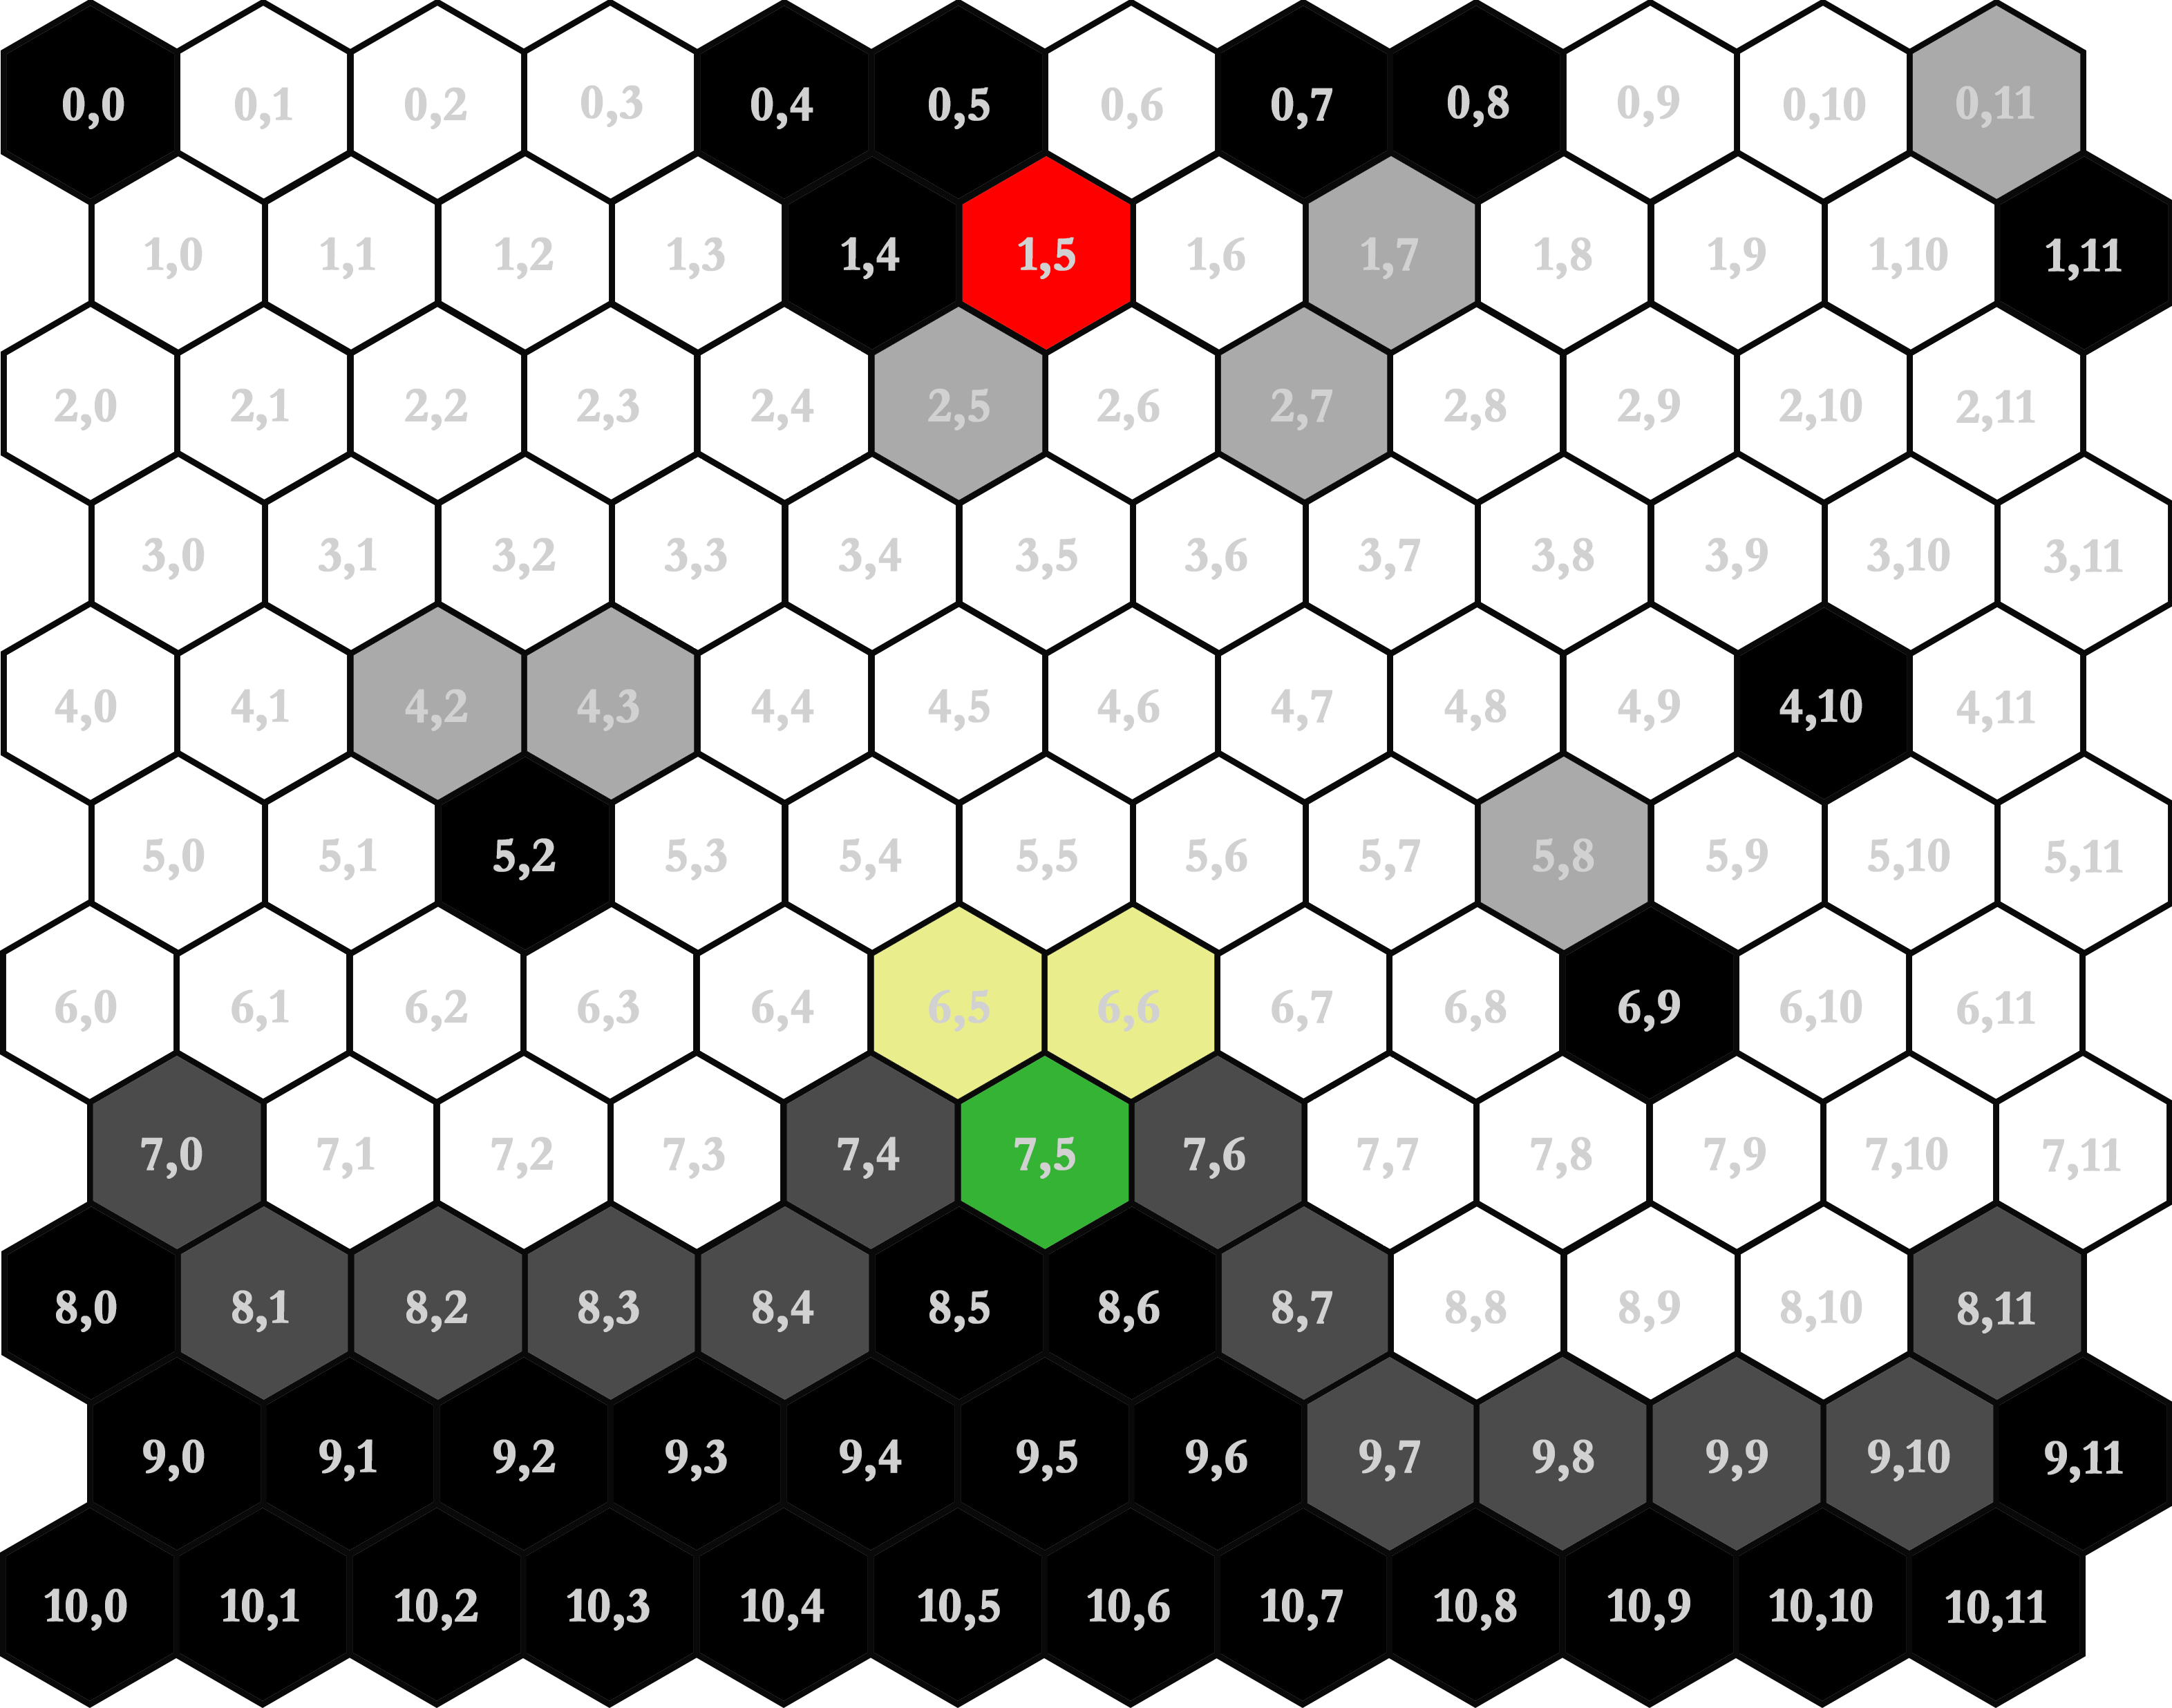
\includegraphics[width = 0.70\textwidth]{./maps/c315.png}
}
\end{center}

\subsection*{Setup Instructions}
\begin{itemize}
\item \textbf{Goldenrod:} Character Start Location. Place the character on either tile.
\item \textbf{Red:} Enemy Start Location.
\item \textbf{Black:} Impassable Boundary/Full-Cover
\item \textbf{Dark Gray:} Pitfall. Any entity that enters this tile is defeated.
\item \textbf{Light Gray:} Half-Cover.
\item \textbf{Green:} Escape Tile.
\end{itemize}

\pagebreak

\subsection*{Victory}
The Thing falls to its knees--or the closest anatomical feature that could be described as such. In a pose reminiscent of a drunkard’s morning-after, it issues a few, wet coughs and then spews forth a stream of molten bile. After one last spurt, the Thing collapses into the pool of its own ichor. Its barklike skin sizzles and pops, giving off a rancid smell redolent of a tannery.\\

You have no word with which to describe the creature you’ve just slain. Your eyes likely never beheld such a thing, in this life or any other. But some of its features were... human in appearance, and disturbingly so.\\

On closer inspection, the “nest” of burnt corpses contains both prisoner and guards. Their arms and legs have been broken and entwined, as if the Thing meant to weave them into a quilt. One peculiar man catches your eye. He clearly wasn’t a prisoner, and yet he wasn’t wearing a guard’s uniform either. He’s a recent addition to the pile; most of his gear is still in good condition. His leather chestpiece is sewn with an emblem of a golden hand.\\

>> Nest of Souls (20)\\
\gain{Travelling Leathers Set}\\
\gain{Stiletto}\\
\gain{Main-Gauche}\\
\gain{Throwing Knives}\\
>> \turnto{c316}

\subsection*{Defeat}
The fight passes in a blur, leaving you with only a single memory of the ordeal: its searing pain. You stumble backwards and try to regain your footing, but your foot finds no purchase--only air. There is a brief moment of terror as you slip from the mezzanine, and tumble down the rubble to the cell block below. At the bottom of the slope, you raise your head to discover a pulsing, red glow making its way down into the fog. You manage to struggle to your feet, and limp across the common area to the safety of the security hallway. Once inside, you wrestle with the lever until the main doors close, and collapse against a wall.\\

When you awaken, the scorchmarks streaking across the walls take on a new and terrifying meaning.\\

>> Clear all \textbf{HP} slots\\
>> \textbf{HMN} - 1\\
>> \turnto{c35}

\subsection*{Retreat}
It’s too late to do anything for the comrades of this cell block, but you resolve not to join them in that horrendous nest. The least you can do is survive.\\

You flee down the slope and across the common area to the safety of the security hallway. A glance over your shoulder reveals a pulsing, red glow bounding through the fog after you. Once inside, you wrestle with the lever until the main doors close.\\

>> Clear all \textbf{HP} slots\\
>> \turnto{c35}
